\documentclass[11pt]{article}
\usepackage{enumerate}
\usepackage{fullpage}
\usepackage{fancyhdr}
\usepackage{amsmath, amsfonts, amsthm, amssymb}
\usepackage{color}
\usepackage[]{graphicx}

\setlength{\parindent}{0pt}
\setlength{\parskip}{5pt plus 1pt}
\pagestyle{empty}

\def\indented#1{\list{}{}\item[]}
\let\indented=\endlist

\newcounter{questionCounter}
\newcounter{partCounter}[questionCounter]
\newenvironment{question}[2][\arabic{questionCounter}]{%
    \setcounter{partCounter}{0}%
    \vspace{.25in} \hrule \vspace{0.5em}%
        \noindent{\bf #2}%
    \vspace{0.8em} \hrule \vspace{.10in}%
    \addtocounter{questionCounter}{1}%
}{}
\renewenvironment{part}[1][\alph{partCounter}]{%
    \addtocounter{partCounter}{1}%
    \vspace{.10in}%
    \begin{indented}%
       {\bf (#1)} %
}{\end{indented}}

%%%%%%%%%%%%%%%%%%%%%%%HEADER%%%%%%%%%%%%%%%%%%%%%%%%%%%%%%
\newcommand{\myname}{Shashank Singh}
\newcommand{\myandrew}{sss1@andrew.cmu.edu}
\newcommand{\myclass}{86-595 Neural Data Analysis}
\newcommand{\myhwnum}{3}
\newcommand{\duedate}{Tuesday, October 9, 2012}
%%%%%%%%%%%%%%%%%%%%%%%%%%%%%%%%%%%%%%%%%%%%%%%%%%%%%%%%%%%

%%%%%%%%%%%%%%%%%%%%CONTENT MACROS%%%%%%%%%%%%%%%%%%%%%%%%%
\newcommand{\be}{\begin{enumerate}}
\newcommand{\ee}{\end{enumerate}}
\renewcommand{\qed}{\quad $\blacksquare$}
\newcommand{\mqed}{\quad \blacksquare}
\newcommand{\inv}{^{-1}}
\newcommand{\bx}{\mathbf{x}}
\newcommand{\by}{\mathbf{y}}
\newcommand{\bff}{\mathbf{f}}
\newcommand{\bzero}{\mathbf{0}}
\newcommand{\N}{\mathbb{N}} % natural numbers
\newcommand{\Q}{\mathbb{Q}} % rational numbers
\newcommand{\R}{\mathbb{R}} % real numbers
\newcommand{\E}[1]{\mathsf{E}\left[#1\right]} % expected value
\newcommand{\Var}[1]{\mathsf{Var}\left[#1\right]} % variance
\newcommand{\Poisson}[1]{\operatorname{Poisson}\left(#1\right)} % Poisson distribution
\newcommand{\Exp}[1]{\operatorname{Exp}\left(#1\right)} % Exponential distribution
\newcommand{\U}[2]{\operatorname{U}\left(#1,#2\right)} % Uniform distribution
\newcommand{\Bern}[1]{\operatorname{Bernoulli}\left( #1 \right)} % Bernoulli distribution
\newcommand{\pr}[1]{\mathsf{P}\left( #1 \right)} % probability of event #1
\newcommand{\argmax}{\operatorname{argmax}}
%%%%%%%%%%%%%%%%%%%%%%%%%%%%%%%%%%%%%%%%%%%%%%%%%%%%%%%%%%%

\begin{document}
\thispagestyle{plain}

{\Large Homework \myhwnum} \\
\myclass \\
Name: \myname \\
Email: \myandrew \\
Due: \duedate \\
\begin{question}{Problem 1}
See last few pages for MATLAB code used for each part.
\begin{enumerate}[a.]
\item
See Figure~\ref{fig:1a}.
\begin{figure}[h]
\begin{center}
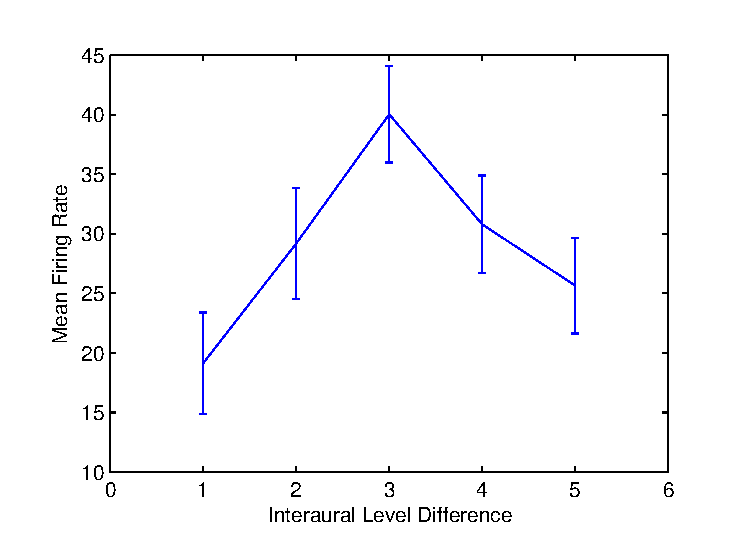
\includegraphics[width=0.46\textwidth]{1a}
\end{center}
\caption{Error bars denote one standard deviation from the mean.}
\label{fig:1a}
\end{figure}

\item
See Figure~\ref{fig:1b}.
\begin{figure}[h]
\begin{center}
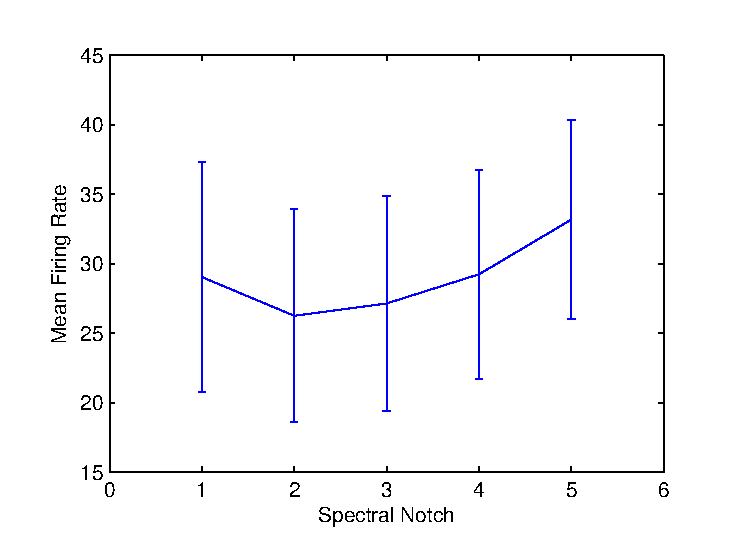
\includegraphics[width=0.46\textwidth]{1b}
\end{center}
\caption{Error bars denote one standard deviation from the mean.}
\label{fig:1b}
\end{figure}

\item
See Figure~\ref{fig:1c}.
\begin{figure}[h]
\begin{center}
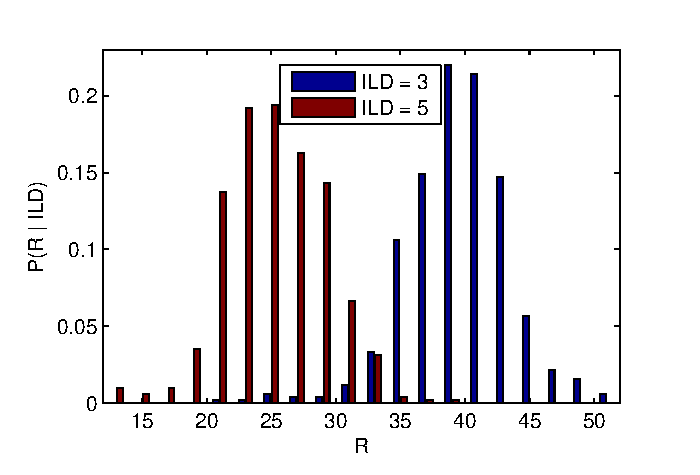
\includegraphics[width=0.46\textwidth]{1c}
\end{center}
\caption{Spike counts were binned in groups of 2.}
\label{fig:1c}
\end{figure}

\item
See Figure~\ref{fig:1d}.
\begin{figure}[h]
\begin{center}
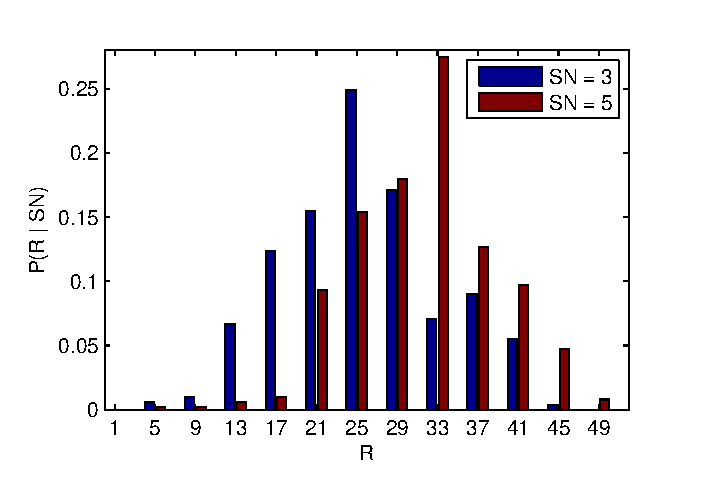
\includegraphics[width=0.46\textwidth]{1d}
\end{center}
\caption{Spike counts were binned in groups of 4.}
\label{fig:1d}
\end{figure}

\item Figures ~\ref{fig:1c} and ~\ref{fig:1d} suggest that spike counts carry
more information about ILD; given a spike count is easy to classify the ILD as
3 or 5, except for trials with 32-33 spikes, which occur are less than 5\% of
trials. On the other hand, there is considerable overlap between the conditional
PDF's of $P(R | SN)$, and, for trials with 21-44 spikes (more than 50\% of
trials), it is difficult to predict whether $SN = 3$ or $SN = 5$ without much
error.

\item Since each $ILD$ and $SN$ occurs with uniform probability $\frac15$, as
shown in Problem 4a. of Homework Set 2,
\[H(ILD) = H(SN) = \log_2(5) \approx \mbox{\fbox{$2.32$.}}\]
$H(R) \approx \mbox{\fbox{$5.0026$}}$ (see code).
As shown in class,
\[MI(R;ILD),MI(R;SN)
 \leq    \min\{H(R),H(ILD)\}
 =       \min\{H(R),H(SN)\}
 \approx \mbox{\fbox{$2.32$.}}\]

\item
$H(R | ILD) \approx \mbox{\fbox{$4.0036$}}$ (see code).
$H(R | SN)  \approx \mbox{\fbox{$4.8344$}}$ (see code).

\item As shown in class,
\[MI(R;ILD)
 =       H(R) - H(R | ILD)
 \approx 5.0026 - 4.0036
 =       \mbox{\fbox{$0.9990$,}}\]
\[MI(R;ILD)
 =       H(R) - H(R |SN)
 \approx 5.0026 - 4.8344
 =       \mbox{\fbox{$0.1682$.}}\]

\end{enumerate}
\end{question}

\begin{question}{Problem 2}
\begin{enumerate}[a.]
\item
See Figure~\ref{fig:2abc}.

\item
See Figure~\ref{fig:2abc}.

\item
See Figure~\ref{fig:2abc}.
\begin{figure}[h]
\begin{center}
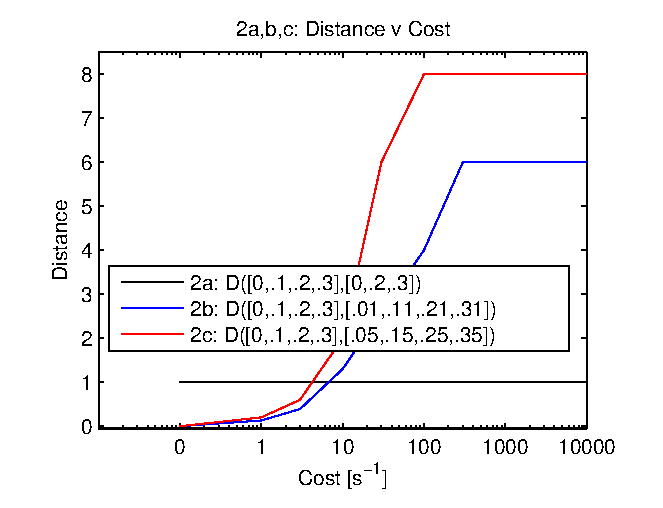
\includegraphics[width=0.46\textwidth]{2abc}
\end{center}
\caption{Plot of VP Distance versus cost.}
\label{fig:2abc}
\end{figure}

\item The mean distance is \fbox{$31.9167$} (see code).
See figure~\ref{fig:2d}.
\begin{figure}[h]
\begin{center}
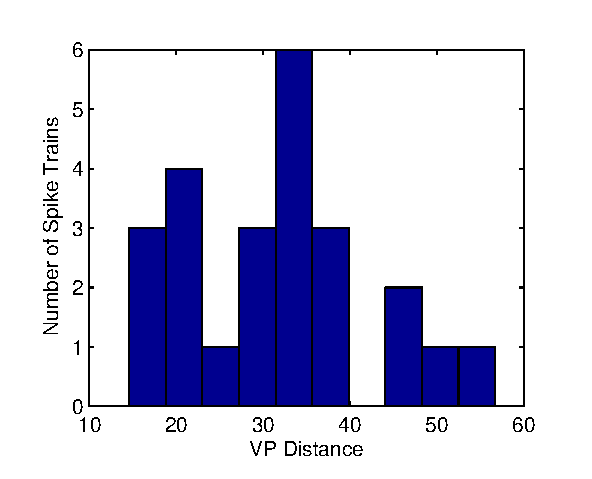
\includegraphics[width=0.46\textwidth]{2d}
\end{center}
\caption{Distribution of VP distances of spikes under identical conditions.}
\label{fig:2d}
\end{figure}

\item The mean distance is \fbox{$32.3364$} (see code). The spike train with
$ILD = SN = trial = 1$ is closer to the $SN = 1$ group than the $SN = 5$
group. See figure~\ref{fig:2e}.
\begin{figure}[h]
\begin{center}
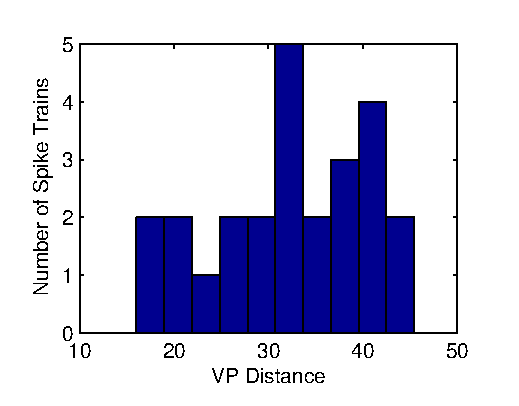
\includegraphics[width=0.46\textwidth]{2e}
\end{center}
\caption{Distribution of VP distances of spikes with $SN = 5$.}
\label{fig:2e}
\end{figure}

\item
\begin{verbatim}
>> confmat_ild{8}

ans =

    25     0     0     0     0
    22     3     0     0     0
    19     0     0     0     6
    18     0     0     1     6
    15     0     0     0    10
\end{verbatim}
Since the entries of \texttt{confmat\_ild\{8\}} do not vary much between the
rows, there should not be much information about ILD.


\item
\begin{verbatim}
>> confmat_sn{8}

ans =

    11    13     1     0     0
     0    23     2     0     0
     0     0    25     0     0
     0     0     7    18     0
     0     0     5     1    19
\end{verbatim}
Since most of the spikes were correctly classified, so that the entries of
\texttt{confmat\_sn\{8\}} lie along the diagonal, there should be a large
amount of information about SN.

\item See figures~\ref{fig:2i1} and \ref{fig:2i2}.
\begin{figure}[h]
\begin{center}
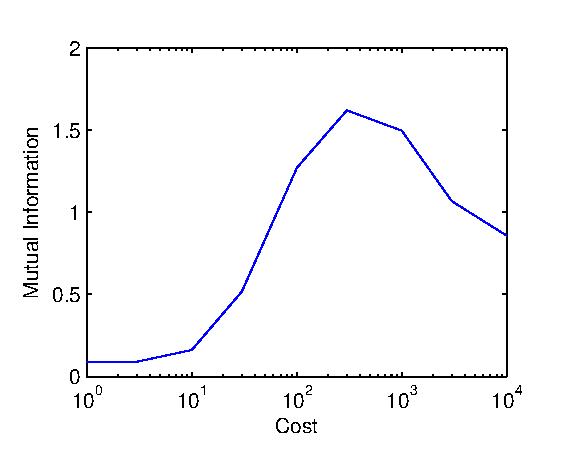
\includegraphics[width=0.46\textwidth]{2i1}
\end{center}
\caption{Mutual information between estimated and actual ILD.}
\label{fig:2i1}
\end{figure}

\begin{figure}[h]
\begin{center}
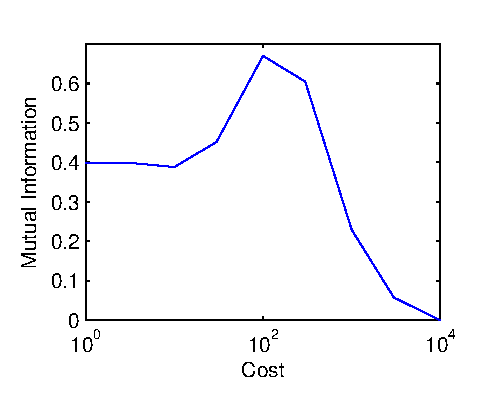
\includegraphics[width=0.46\textwidth]{2i2}
\end{center}
\caption{Mutual information between estimated and actual ILD.}
\label{fig:2i2}
\end{figure}

\item Problem 1 shows that the neuron's spike count primarily carries
ILD information. This is encoded in a tuning curve, and is selective to
$ILD = 3$. Thus, the neuron differentiates $ILD = 3$ from $ILD$ values of
greater or lesser index, although the tuning curve in Figure~\ref{fig:1a}
suggests the neuron's firing rate fails to distinguish well between $ILD = 2$
and $ILD = 4$ or $ILD = 1$ and $ILD = 5$. Figure~\ref{fig:1b} shows that the
neuron's spike count is essentially independent of $SN$, and, indeed,
Figure~\ref{fig:1d} showed that $SN$ cannot be accurately determined from
spike count. Finally, the mutual information between spike count and $ILD$ was
shown to be about $6$ times that between spike count and $SN$.

Problem 2 showed that the neuron's spike timing primarily carries SN
information. For large costs, there is little or no correlation between $ILD$
and estimated $ILD$, because the VP metric places too much value on precise
spike timing to accurately measure the distance between train. This is not
true, however, for $SN$, which can be measured reasonably well with a cost of
$q = 10^3$, and even somewhat with a cost of $q = 10^4$.
\end{enumerate}
\end{question}

\begin{question}{Problem 3}
Computing the confusion matrices in part 2h. took quite a while, but probably
just because I need to brush up on my matlab. Overall, this homework took a
lot longer than the previous two assignments; I think theory tends to be much
easier (or at least, much less time consuming) than the programming. However,
most of Problem 1 also went pretty quickly.

Problem 2, especially parts g-i, definately taught me the most. It was
interesting to use the VP distance to classify spike trains based on their
estimated stimuli. It was also helpful, in Problem 1, to apply some
information theory to actual data, although 1g was a bit tedious, mostly
because the structure of the data was not particularly amenable to the
computation.

Parts a-c of Problem 2 probably taught me the least, but they were also very
quick and easy.
\end{question}

\newpage
\section*{Code}

\begin{question}{Problem 1}
\begin{enumerate}[a.]
\item
\begin{verbatim}
>> for i=1:5
     for j=1:5
       for k=1:102
         d(i,j,k) = length(find(snild_dat(:,1) ==  i ...
                              & snild_dat(:,2) ==  j ...
                              & snild_dat(:,3) ==  k));
       end
     end
   end
>> c = reshape(d,[5 5*102]);
>> errorbar(1:5,mean(c,2),std(c,0,2));
\end{verbatim}

\item
\begin{verbatim}
>> c = reshape(permute(d, [2 1 3]),[5 5*102]);
>> errorbar(1:5,mean(c,2),std(c,0,2));
\end{verbatim}

\item
\begin{verbatim}
>> c = reshape(d,[5 5*102]);
>> x(1,:) = histc(c(3,:),1:2:52); x(2,:) = histc(c(5,:),1:2:52);
>> x(1,:) = x(1,:) ./ sum(x(1,:)); x(2,:) = x(2,:) ./ sum(x(2,:));
>> bar(1:2:52,x'); axis([12 52 0 0.23]);
\end{verbatim}

\item
\begin{verbatim}
>> c = reshape(permute(d, [2 1 3]),[5 5*102]);
>> x(1,:) = histc(c(3,:),1:4:52); x(2,:) = histc(c(5,:),1:4:52);
>> x(1,:) = x(1,:) ./ sum(x(1,:)); x(2,:) = x(2,:) ./ sum(x(2,:));
>> bar(1:4:52,x'); axis([12 52 0 0.28]);
\end{verbatim}

\item No code for this part.

\item The following code was used to compute $H(R)$:
\begin{verbatim}
>> c = histc(d(:),unique(d(:)));
>> c = c ./ sum(c);
>> HR = -sum(c .* log2(c));
\end{verbatim}

\item The following code was used to compute $H(R | ILD)$:
\begin{verbatim}
>> c = reshape(d,[5 5*102]);
>> c = histc(c',unique(d(:)))';
>> for i=1:5, ccond(i,:) = c(i,:)./sum(c(i,:)); end
>> plogcond = ccond .* log2(ccond);
>> plogcond(isnan(plogcond) = 0;
>> HR = mean(-sum(plogcond'));
\end{verbatim}
The following code was used to compute $H(R | SN)$:
\begin{verbatim}
>> c = reshape(permute(d, [2 1 3]),[5 5*102]);
>> c = histc(c',unique(d(:)))';
>> for i=1:5, ccond(i,:) = c(i,:)./sum(c(i,:)); end
>> plogcond = ccond .* log2(ccond);
>> plogcond(isnan(plogcond) = 0;
>> HR = mean(-sum(plogcond'));
\end{verbatim}
\item No code for this part.

\end{enumerate}
\end{question}

\begin{question}{Problem 2}
\begin{enumerate}[a.]
\item The following code was use to calculate \texttt{dist\_2a}
\begin{verbatim}
>> costs = [0,1,3,10,30,100,300,1000,3000,10000];                              
>> spike_train_1 = [0, 0.1, 0.2, 0.3];                                         
>> spike_train_2 = [0, 0.2, 0.3];     
>> for i=1:10, dist_2a(i) = HW3_spkd(spike_train_1,spike_train_2,costs(i)); end
\end{verbatim}

\item
\begin{verbatim}
>> spike_train_2 = [0.1, 0.11, 0.21, 0.31];
>> for i=1:10, dist_2b(i) = HW3_spkd(spike_train_1,spike_train_2,costs(i)); end
\end{verbatim}

\item
\begin{verbatim}
>> spike_train_2 = [0.05, 0.15, 0.25, 0.35];                                 
>> for i=1:10, dist_2c(i) = HW3_spkd(spike_train_1,spike_train_2,costs(i)); end
\end{verbatim}

\item
\begin{verbatim}
>> for i=1:5
     for k=1:5
       trains{i,k} = snild_dat2(find(snild_dat2(:,1) ==  i
                                   & snild_dat2(:,2) ==  1
                                   & snild_dat2(:,3) ==  k),4);
     end
   end
>> trains = trains(:);
>> train1 = trains{1};
>> for i = 2:length(trains)
     dist(i-1) = HW3_spkd(train1,train{i},1000);
   end
>> meandist = mean(dist);
\end{verbatim}

\newpage
\item
\begin{verbatim}
>> for i=1:5
     for k=1:5
       trains{i,k} = snild_dat2(find(snild_dat2(:,1) ==  i
                                   & snild_dat2(:,2) ==  5
                                   & snild_dat2(:,3) ==  k),4);
     end
   end
>> trains = trains(:);
>> for i = 1:length(trains)
     dist(i) = HW3_spkd(train1,train{i},1000);
   end
>> meandist = mean(dist);
\end{verbatim}

\item The following code was used to compute each confusion matrix:
\begin{verbatim}
function cf = confmat(snild_dat,cost)
  cf = zeros(5,5);
  trains = cell(5,5,5);

  for i=1:5
    for j=1:5
      for k=1:5
        trains{i,j,k} = snild_dat(find(snild_dat(:,1) ==  i
                                     & snild_dat(:,2) ==  j
                                     & snild_dat(:,3) ==  k),4);
      end
    end
  end

  dists = zeros(5,5,5);
  for i=1:5 % current ILD
    for j=1:5 % current SN
      for k=1:5 % current trial

        for x=1:5 % comparison ILD
          for y=1:5 % comparison SN
            for z=1:5 %comparison trial
              dists(x,y,z) = HW3_spkd(trains{i,j,k},trains{x,y,z},cost);
            end
          end
        end
        mean_dists = mean(mean(dists,3),2);
        [~, assignment] = min(mean_dists);
        cf(i,assignment) = cf(i,assignment) + 1;
      end
    end
  end
end

\end{verbatim}

\item The same code was used as in part f., except that the ILD and SN columns
of \texttt{snild\_dat} were swapped.

%TODO
\item The following code was used to compute each mutual information value for
ILD (the code used for SN was essentially identical):
\begin{verbatim}
>> for i=1:10
     confmat_ild{i} = confmat_ild{i} ./ sum(sum(confmat_ild{i}));
   end
>> for q=1:10
     for i=1:5
       for j=1:5
         mi(i,j) = confmat_ild{q}(i,j) .* log2(confmat_ild{q}(i,j) ...
                                        ./ (0.2 .* sum(confmat_ild{q}(:,j))));
         mi(isnan(mi)) = 0;
       end
     end
     MI(q)=sum(mi(:));
   end
\end{verbatim}

\item No code for this part.

\end{enumerate}
\end{question}
\end{document}
